\documentclass[a4paper]{article}
\usepackage[utf8]{inputenc}
\usepackage[spanish, es-tabla, es-noshorthands]{babel}
\usepackage[table,xcdraw]{xcolor}
\usepackage[a4paper, footnotesep = 1cm, width=20cm, top=2.5cm, height=25cm, textwidth=18cm, textheight=25cm]{geometry}
%\geometry{showframe}

\usepackage{tikz}
\usepackage{amsmath}
\usepackage{amsfonts}
\usepackage{amssymb}
\usepackage{float}
\usepackage{graphicx}
\usepackage{caption}
\usepackage{subcaption}
\usepackage{multicol}
\usepackage{multirow}
\setlength{\doublerulesep}{\arrayrulewidth}
\usepackage{booktabs}
\usepackage{mathrsfs,amsmath}
\usepackage{hyperref}
\hypersetup{
    colorlinks=true,
    linkcolor=blue,
    filecolor=magenta,      
    urlcolor=blue,
    citecolor=blue,    
}

\newcommand{\quotes}[1]{``#1''}
\usepackage{array}
\newcolumntype{C}[1]{>{\centering\let\newline\\\arraybackslash\hspace{0pt}}m{#1}}
\usepackage[american]{circuitikz}
\usetikzlibrary{calc}
\usepackage{fancyhdr}
\usepackage{units} 

\graphicspath{./Imagenes}

\pagestyle{fancy}
\fancyhf{}
\lhead{22.05 ASSD}
\rhead{Mechoulam, Lambertucci, Rodriguez, Londero}
\rfoot{Página \thepage}

\begin{document}
El modulo de \textbf{Sample and Hold}  puede ser esquematizado de la siguiente forma:

\begin{figure}[H]
	\centering
	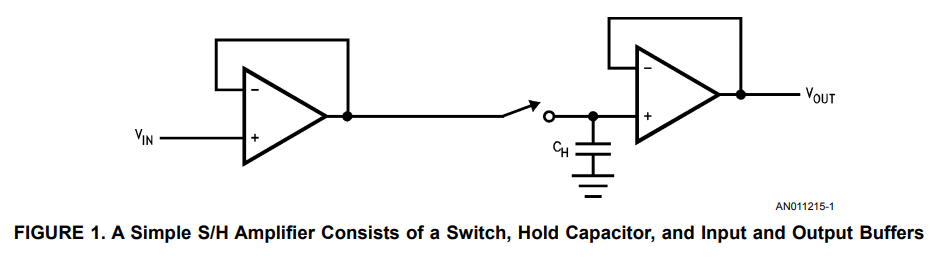
\includegraphics[width=0.7\linewidth]{ImagenesEjercicio4/SyH}
	\caption{}
	\label{fig:syh}
\end{figure}

Su objetivo es el de muestrear la señal analógica de entrada y retener su valor por un pequeño intervalo de tiempo para que la circuiteria colocada inmediatamente después puede utilizar ese valor.

 Sin embargo, es necesario adaptarlo a las condiciones en las que se lo va a utilizar. Para esto, se incluyen pines de corrección de tensión de offset, selección tasa de muestreo y finalmente otro muy importante para escoger el capacitor, $C_{hold}$ más apropiado.
 
 \subsubsection{Circuito de corrección de offset}
 Al diseñar un circuito siempre se debe tener que los procesos de fabricación no son perfectos. En el caso de la digitalización de señales las tensiones de offset pueden provocar interpretaciones erróneas de los verdaderos valores de la señal. De hecho se recomienda que la tensión de offset este por debajo de la mitad del voltaje que ofrece el LSB.
 $$
 V_{OS} < \frac{FS}{2^{n+1}} 
 $$
Donde \textit{n }es la resolución del \textbf{ADC}
y \textit{FS} es el tope de escala.

El fabricante nos brinda una configuración para poder compensar la tensión de offset:
\begin{figure}[H]
	\centering
	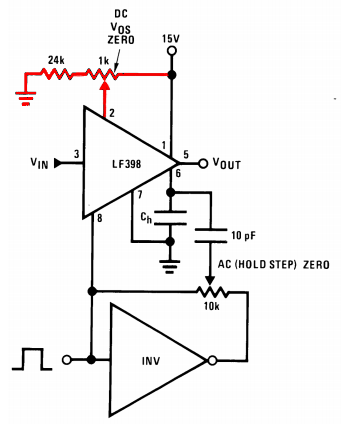
\includegraphics[scale=0.6]{ImagenesEjercicio4/DCcolorized}
	\caption{En \color[red]{rojo}}
	\label{fig:dccolorized}
\end{figure}


\end{document}